
\section{Annotation Quality} 
\label{sec:Annotation Quality}


\subsection{How precise are the temporal annotations?}
\label{sec:Annotation Quality:a1}
Since we did not have any ground truth for when events occur within the files, we simply compared temporal differences of annotations from different annotators corresponding to the same region. A pair of annotations were said to correspond to the same region if both their respective onset and offset times separately do not deviate by more than 0.5 seconds. This of course introduces a trade-off between False Positives and False Negatives.
Then, the absolute differences in onset-/offset times and durations were gathered and plotted in histograms, shown in Figure ~\ref{fig:2_a}.\\
We can see that most annotations fall below a difference in onset-/offset times of 0.1 seconds. Depending on the temporal resolution of the audio features, this might actually lead to some wrongly predicted frames in the future. Overall, most annotations seem to be pretty accurate.

\begin{figure}[htbp]
  \centering
  \begin{subfigure}[b]{0.33\textwidth}
    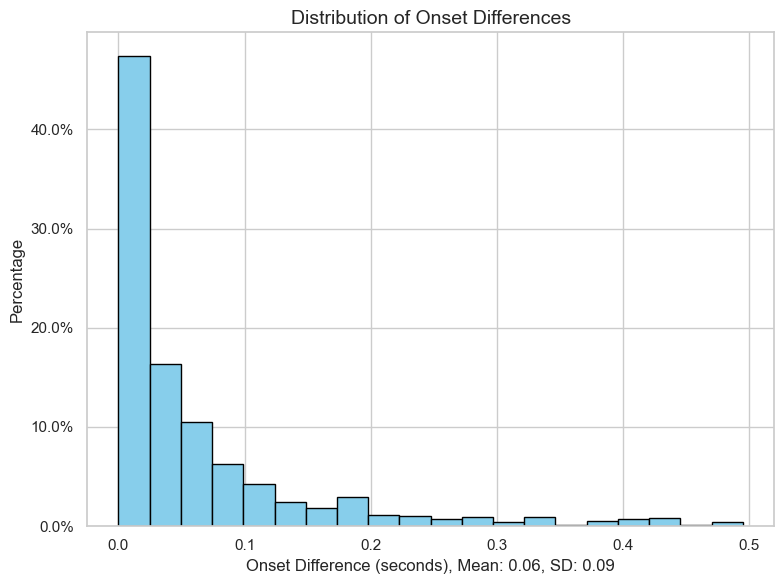
\includegraphics[width=\textwidth, height=4cm]{figs/onset_diffs.png}
  \end{subfigure}
  \hfill
  \begin{subfigure}[b]{0.33\textwidth}
    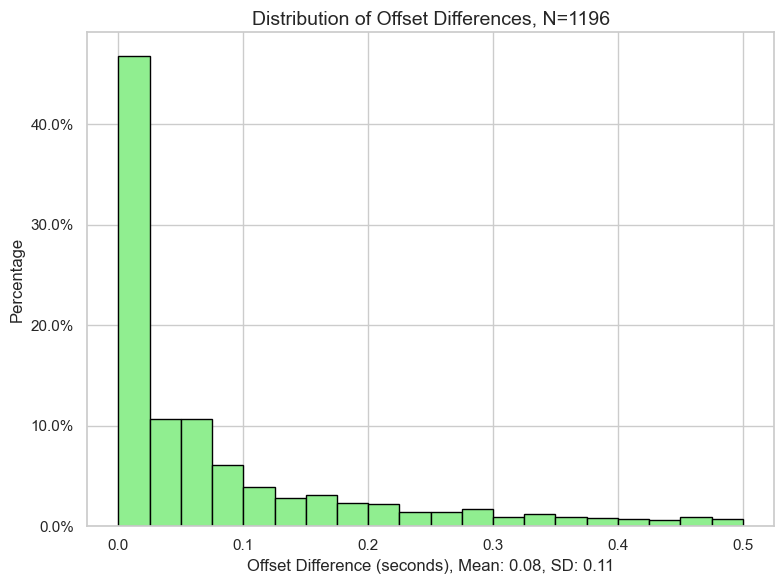
\includegraphics[width=\textwidth, height=4cm]{figs/offset_diffs.png}
  \end{subfigure}
  \hfill
  \begin{subfigure}[b]{0.33\textwidth}
    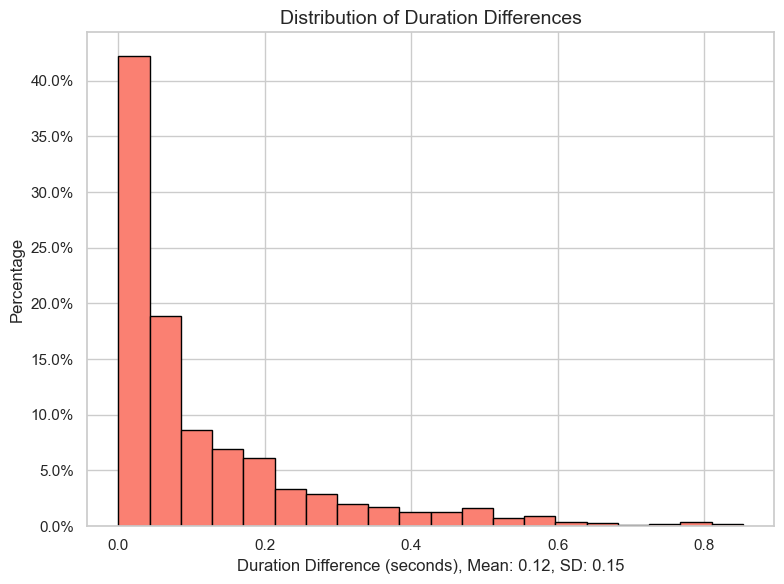
\includegraphics[width=\textwidth, height=4cm]{figs/duration_diffs.png}
  \end{subfigure}
  \caption{Absolute differences in onset-/offset times and durations for annotations corresponding to the same regions.}
  \label{fig:2_a}
\end{figure}

\subsection{How similar are the text annotations that correspond to the same region?}
\label{sec:Annotation Quality:b1}
Using the same criterion as described above, we collected pairs of annotations corresponding to the same regions. For each of these pairs we then simply fetched their annotation text embeddings and calculated their cosine-similarity. The results can be seen in Figure ~\ref{fig:2_b}. \\
We definitely see a similarity between the texts, as the bulk of the similarities lies above 0. We were a bit surprised that the average similarity is only 0.44, as we expected it to be way higher. We even found some similarities < 0, which might be the results of annotations containing false information.

\begin{figure}[htbp]
  \centering
  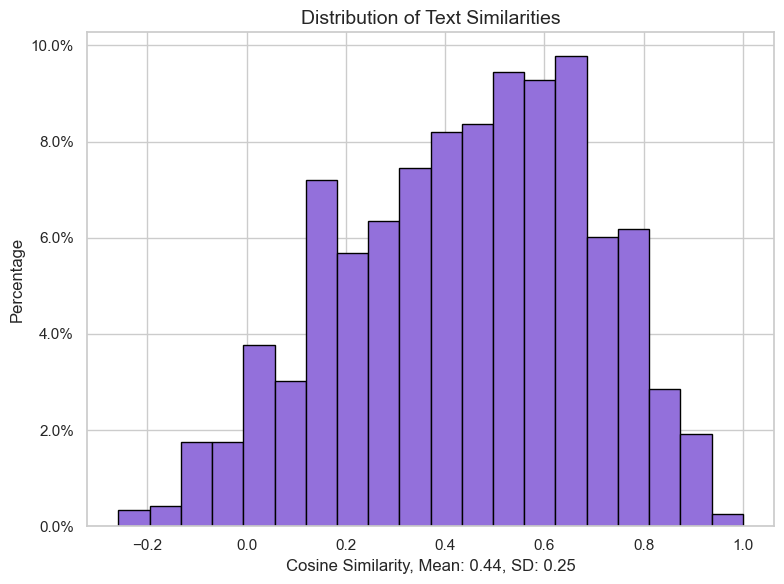
\includegraphics[width=0.5\textwidth, height=4cm]{figs/sim_diffs.png}
  \caption{Cosine similarities between annotations corresponding to the same regions.}
  \label{fig:2_b}
\end{figure}

\subsection{How many annotations did we collect per file? How many distinct sound events per file?}
\label{sec:Annotation Quality:a2}
The number of annotations per file was easily calculated by grouping the corresponding dataframe by filenames.\\
Estimating the number of distinct sound events per file was a bit more complicated. For each of $N$ annotations from one annotator for one file, we fetched the corresponding annotation embeddings and computed their pairwise cosine similarities. They were then put into a $N \times N$ similarity matrix. This matrix was then filtered such that all values below a similarity threshold of 0.8 were set to 0 and all others to 1 to turn the matrix into. This then gives connected components within the graph corresponding to that matrix where the annotations are extremely similar, most likely because they describe the same sound event. Therefore the number of connected components is our estimate for the number of distinct sound events. If there were multiple annotators per file, the number was averaged and rounded. The results are shown in Figure ~\ref{fig:2_c}. \\
The results seem reasonable. We have an average of 3.97 annotations and 2.23 distinct sound events per file.

\begin{figure}[htbp]
  \centering
  \begin{subfigure}[b]{0.49\textwidth}
    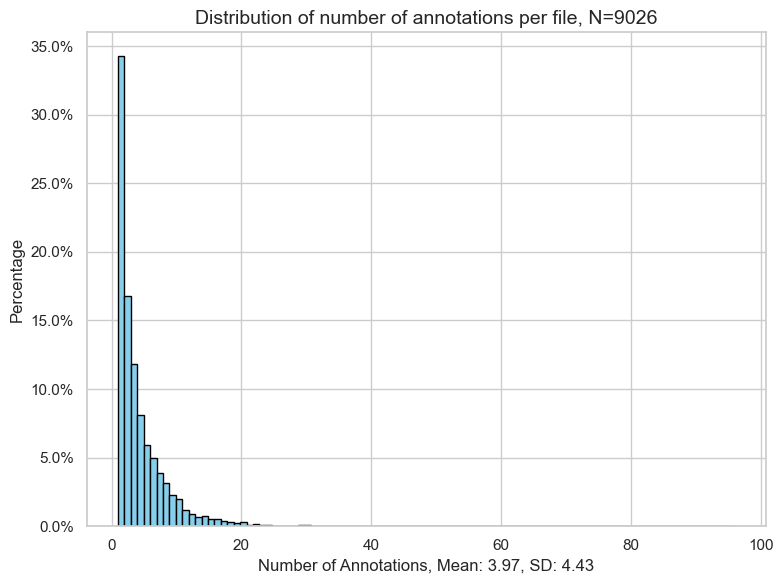
\includegraphics[width=\textwidth, height=4cm]{figs/annotation_dist.png}
  \end{subfigure}
  \hfill
  \begin{subfigure}[b]{0.49\textwidth}
    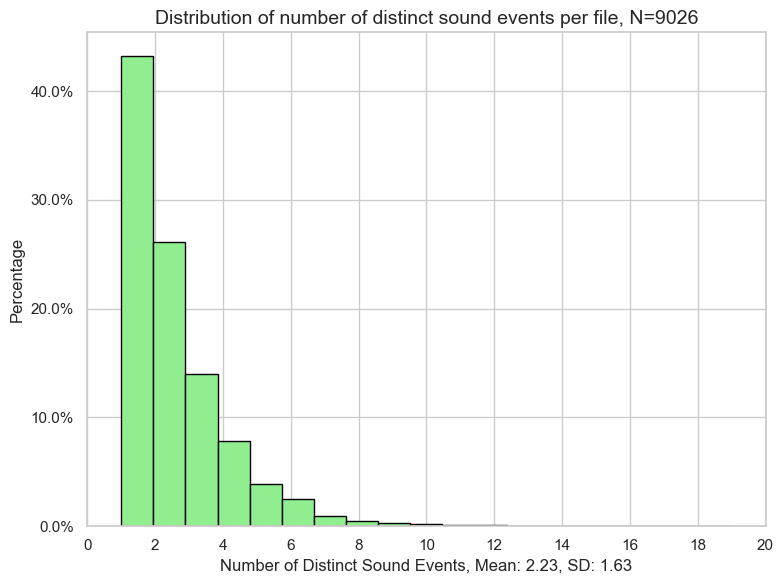
\includegraphics[width=\textwidth, height=4cm]{figs/sound_event_dist.png}
  \end{subfigure}
  \caption{Distributions of annotations and distinct sound events per file.}
  \label{fig:2_c}
\end{figure}

\subsection{How detailed are the text annotations? How much does the quality of annotations vary between
different annotators?}
\label{sec:Annotation Quality:b2}
As quality metrics for a single annotation,we decided to compare the Text-Token-Ratio (TTR, number of unique word divided by the number of words), the number of spelling errors (using a simple off-the-shelf spell checker) and the number of words. Analyzing the textual annotations for different annotators led us to the following Figure ~\ref{fig:2_d}.\\
The best metric out of these for checking how detailed the annotations are would most likely be the number of words per annotation. As the average annotator has written an average of 7.85 words per annotation, most of them seem to be reasonably detailed.
As for the variation in annotation quality: we were surprised to see that almost half of the annotators had on average more than 1 spelling error in their annotation. There also seem to be some with extremely low word counts. The standard deviation 3.53 for the average number of words seems reasonable as well. Most annotations should be of sufficient quality.
TTR turned out to be mostly useless, as most annotations are so short that it would be very hard to find duplicate words.

\begin{figure}[htbp]
  \centering
  \begin{subfigure}[b]{0.33\textwidth}
    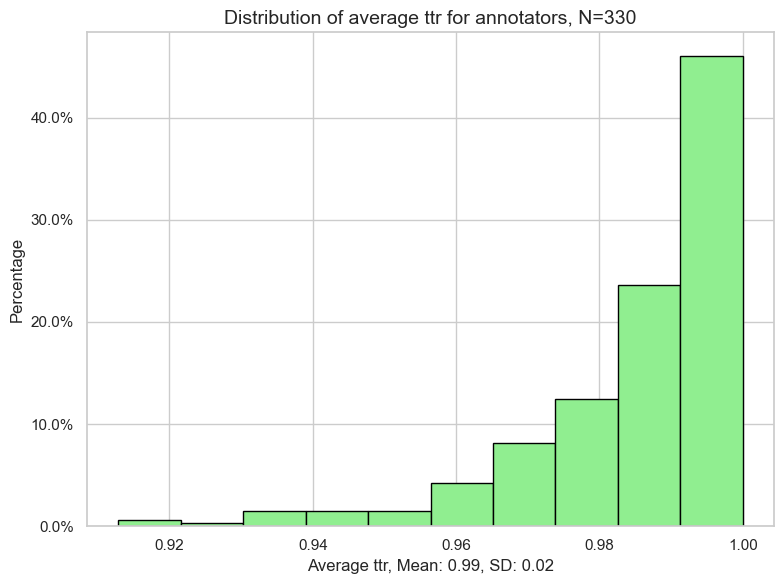
\includegraphics[width=\textwidth, height=4cm]{figs/ttr_dist.png}
  \end{subfigure}
  \hfill
  \begin{subfigure}[b]{0.33\textwidth}
    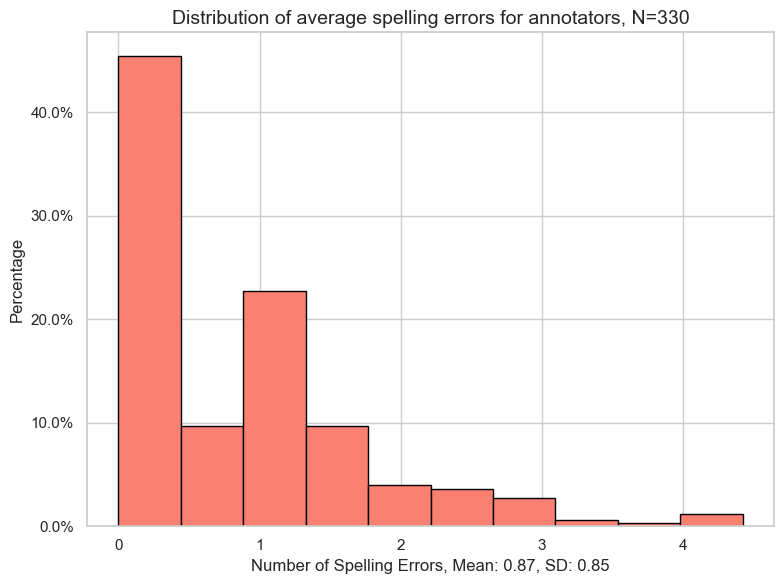
\includegraphics[width=\textwidth, height=4cm]{figs/error_dist.png}
  \end{subfigure}
  \hfill
  \begin{subfigure}[b]{0.33\textwidth}
    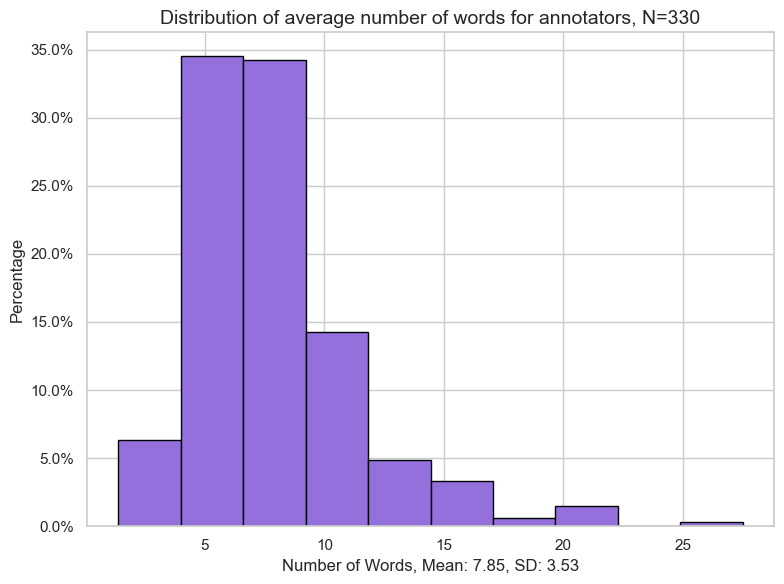
\includegraphics[width=\textwidth, height=4cm]{figs/word_dist.png}
  \end{subfigure}
  \caption{Distributions of quality metrics over all annotators.}
  \label{fig:2_d}
\end{figure}

\subsection{Are there any obvious inconsistencies, outliers, or poor-quality annotations in the data? Propose a
simple method to filter or fix incorrect or poor-quality annotations (e.g., remove outliers, typos, or
spelling errors).}
\label{sec:Annotation Quality:c2}
As our previous analysis has shown: yes, there are some poor quality annotations, i.e. outliers. This may be some consisting only of a single word or not relating to the audio because of some misconception. 
These could simply be removed by checking the word count of the annotations and removing the ones for which the text embedding is really dissimilar from metadata embeddings.
When it comes to fixing typos and spelling errors, one could simply use an off-the-shelf library to go over the texts and correct them.
